% Created by tikzDevice version 0.12 on 2019-04-27 00:00:36
% !TEX encoding = UTF-8 Unicode
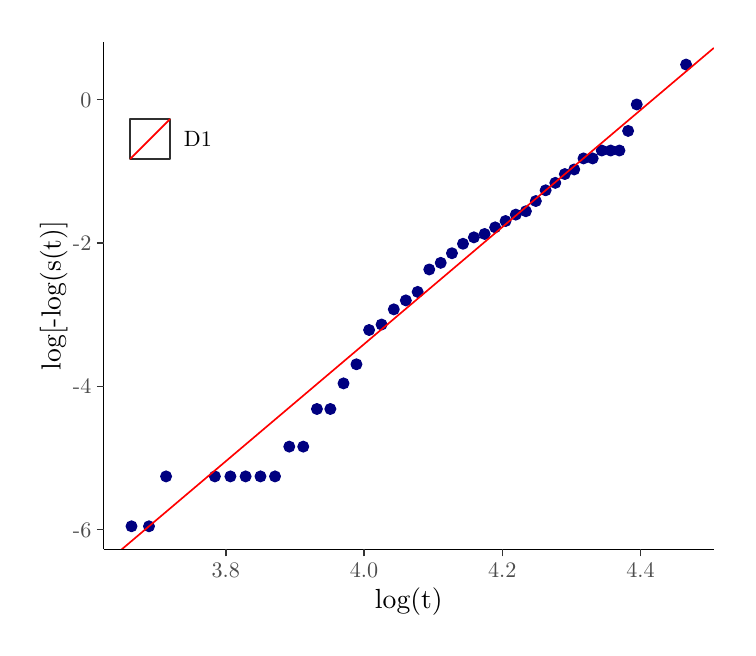
\begin{tikzpicture}[x=1pt,y=1pt]
\definecolor{fillColor}{RGB}{255,255,255}
\path[use as bounding box,fill=fillColor,fill opacity=0.00] (0,0) rectangle (252.94,216.81);
\begin{scope}
\path[clip] (  0.00,  0.00) rectangle (252.94,216.81);
\definecolor{drawColor}{RGB}{255,255,255}
\definecolor{fillColor}{RGB}{255,255,255}

\path[draw=drawColor,line width= 0.5pt,line join=round,line cap=round,fill=fillColor] ( -0.00,  0.00) rectangle (252.95,216.81);
\end{scope}
\begin{scope}
\path[clip] ( 27.50, 28.28) rectangle (247.95,211.81);
\definecolor{fillColor}{RGB}{255,255,255}

\path[fill=fillColor] ( 27.50, 28.28) rectangle (247.95,211.81);
\definecolor{drawColor}{RGB}{0,0,128}
\definecolor{fillColor}{RGB}{0,0,128}

\path[draw=drawColor,line width= 0.4pt,line join=round,line cap=round,fill=fillColor] ( 37.52, 36.63) circle (  1.96);

\path[draw=drawColor,line width= 0.4pt,line join=round,line cap=round,fill=fillColor] ( 43.84, 36.63) circle (  1.96);

\path[draw=drawColor,line width= 0.4pt,line join=round,line cap=round,fill=fillColor] ( 50.01, 54.66) circle (  1.96);

\path[draw=drawColor,line width= 0.4pt,line join=round,line cap=round,fill=fillColor] ( 67.65, 54.66) circle (  1.96);

\path[draw=drawColor,line width= 0.4pt,line join=round,line cap=round,fill=fillColor] ( 73.26, 54.66) circle (  1.96);

\path[draw=drawColor,line width= 0.4pt,line join=round,line cap=round,fill=fillColor] ( 78.75, 54.66) circle (  1.96);

\path[draw=drawColor,line width= 0.4pt,line join=round,line cap=round,fill=fillColor] ( 84.12, 54.66) circle (  1.96);

\path[draw=drawColor,line width= 0.4pt,line join=round,line cap=round,fill=fillColor] ( 89.38, 54.66) circle (  1.96);

\path[draw=drawColor,line width= 0.4pt,line join=round,line cap=round,fill=fillColor] ( 94.53, 65.42) circle (  1.96);

\path[draw=drawColor,line width= 0.4pt,line join=round,line cap=round,fill=fillColor] ( 99.58, 65.42) circle (  1.96);

\path[draw=drawColor,line width= 0.4pt,line join=round,line cap=round,fill=fillColor] (104.52, 79.02) circle (  1.96);

\path[draw=drawColor,line width= 0.4pt,line join=round,line cap=round,fill=fillColor] (109.37, 79.02) circle (  1.96);

\path[draw=drawColor,line width= 0.4pt,line join=round,line cap=round,fill=fillColor] (114.13, 88.27) circle (  1.96);

\path[draw=drawColor,line width= 0.4pt,line join=round,line cap=round,fill=fillColor] (118.80, 95.17) circle (  1.96);

\path[draw=drawColor,line width= 0.4pt,line join=round,line cap=round,fill=fillColor] (123.38,107.56) circle (  1.96);

\path[draw=drawColor,line width= 0.4pt,line join=round,line cap=round,fill=fillColor] (127.88,109.54) circle (  1.96);

\path[draw=drawColor,line width= 0.4pt,line join=round,line cap=round,fill=fillColor] (132.30,115.02) circle (  1.96);

\path[draw=drawColor,line width= 0.4pt,line join=round,line cap=round,fill=fillColor] (136.65,118.26) circle (  1.96);

\path[draw=drawColor,line width= 0.4pt,line join=round,line cap=round,fill=fillColor] (140.92,121.33) circle (  1.96);

\path[draw=drawColor,line width= 0.4pt,line join=round,line cap=round,fill=fillColor] (145.12,129.44) circle (  1.96);

\path[draw=drawColor,line width= 0.4pt,line join=round,line cap=round,fill=fillColor] (149.25,131.83) circle (  1.96);

\path[draw=drawColor,line width= 0.4pt,line join=round,line cap=round,fill=fillColor] (153.31,135.30) circle (  1.96);

\path[draw=drawColor,line width= 0.4pt,line join=round,line cap=round,fill=fillColor] (157.30,138.72) circle (  1.96);

\path[draw=drawColor,line width= 0.4pt,line join=round,line cap=round,fill=fillColor] (161.24,141.04) circle (  1.96);

\path[draw=drawColor,line width= 0.4pt,line join=round,line cap=round,fill=fillColor] (165.11,142.26) circle (  1.96);

\path[draw=drawColor,line width= 0.4pt,line join=round,line cap=round,fill=fillColor] (168.92,144.65) circle (  1.96);

\path[draw=drawColor,line width= 0.4pt,line join=round,line cap=round,fill=fillColor] (172.68,146.94) circle (  1.96);

\path[draw=drawColor,line width= 0.4pt,line join=round,line cap=round,fill=fillColor] (176.38,149.26) circle (  1.96);

\path[draw=drawColor,line width= 0.4pt,line join=round,line cap=round,fill=fillColor] (180.03,150.48) circle (  1.96);

\path[draw=drawColor,line width= 0.4pt,line join=round,line cap=round,fill=fillColor] (183.62,154.16) circle (  1.96);

\path[draw=drawColor,line width= 0.4pt,line join=round,line cap=round,fill=fillColor] (187.16,158.04) circle (  1.96);

\path[draw=drawColor,line width= 0.4pt,line join=round,line cap=round,fill=fillColor] (190.66,160.73) circle (  1.96);

\path[draw=drawColor,line width= 0.4pt,line join=round,line cap=round,fill=fillColor] (194.10,163.91) circle (  1.96);

\path[draw=drawColor,line width= 0.4pt,line join=round,line cap=round,fill=fillColor] (197.50,165.58) circle (  1.96);

\path[draw=drawColor,line width= 0.4pt,line join=round,line cap=round,fill=fillColor] (200.85,169.56) circle (  1.96);

\path[draw=drawColor,line width= 0.4pt,line join=round,line cap=round,fill=fillColor] (204.16,169.56) circle (  1.96);

\path[draw=drawColor,line width= 0.4pt,line join=round,line cap=round,fill=fillColor] (207.43,172.42) circle (  1.96);

\path[draw=drawColor,line width= 0.4pt,line join=round,line cap=round,fill=fillColor] (210.65,172.42) circle (  1.96);

\path[draw=drawColor,line width= 0.4pt,line join=round,line cap=round,fill=fillColor] (213.83,172.42) circle (  1.96);

\path[draw=drawColor,line width= 0.4pt,line join=round,line cap=round,fill=fillColor] (216.97,179.50) circle (  1.96);

\path[draw=drawColor,line width= 0.4pt,line join=round,line cap=round,fill=fillColor] (220.08,189.06) circle (  1.96);

\path[draw=drawColor,line width= 0.4pt,line join=round,line cap=round,fill=fillColor] (237.92,203.47) circle (  1.96);
\definecolor{drawColor}{RGB}{255,0,0}

\path[draw=drawColor,line width= 0.6pt,line join=round] ( 27.50, 22.80) -- (247.95,209.49);
\end{scope}
\begin{scope}
\path[clip] (  0.00,  0.00) rectangle (252.94,216.81);
\definecolor{drawColor}{RGB}{0,0,0}

\path[draw=drawColor,line width= 0.5pt,line join=round] ( 27.50, 28.28) --
	( 27.50,211.81);
\end{scope}
\begin{scope}
\path[clip] (  0.00,  0.00) rectangle (252.94,216.81);
\definecolor{drawColor}{gray}{0.30}

\node[text=drawColor,anchor=base east,inner sep=0pt, outer sep=0pt, scale=  0.80] at ( 23.00, 32.63) {-6};

\node[text=drawColor,anchor=base east,inner sep=0pt, outer sep=0pt, scale=  0.80] at ( 23.00, 84.46) {-4};

\node[text=drawColor,anchor=base east,inner sep=0pt, outer sep=0pt, scale=  0.80] at ( 23.00,136.29) {-2};

\node[text=drawColor,anchor=base east,inner sep=0pt, outer sep=0pt, scale=  0.80] at ( 23.00,188.12) {0};
\end{scope}
\begin{scope}
\path[clip] (  0.00,  0.00) rectangle (252.94,216.81);
\definecolor{drawColor}{gray}{0.20}

\path[draw=drawColor,line width= 0.5pt,line join=round] ( 25.00, 35.38) --
	( 27.50, 35.38);

\path[draw=drawColor,line width= 0.5pt,line join=round] ( 25.00, 87.21) --
	( 27.50, 87.21);

\path[draw=drawColor,line width= 0.5pt,line join=round] ( 25.00,139.04) --
	( 27.50,139.04);

\path[draw=drawColor,line width= 0.5pt,line join=round] ( 25.00,190.88) --
	( 27.50,190.88);
\end{scope}
\begin{scope}
\path[clip] (  0.00,  0.00) rectangle (252.94,216.81);
\definecolor{drawColor}{RGB}{0,0,0}

\path[draw=drawColor,line width= 0.5pt,line join=round] ( 27.50, 28.28) --
	(247.95, 28.28);
\end{scope}
\begin{scope}
\path[clip] (  0.00,  0.00) rectangle (252.94,216.81);
\definecolor{drawColor}{gray}{0.20}

\path[draw=drawColor,line width= 0.5pt,line join=round] ( 71.60, 25.78) --
	( 71.60, 28.28);

\path[draw=drawColor,line width= 0.5pt,line join=round] (121.55, 25.78) --
	(121.55, 28.28);

\path[draw=drawColor,line width= 0.5pt,line join=round] (171.51, 25.78) --
	(171.51, 28.28);

\path[draw=drawColor,line width= 0.5pt,line join=round] (221.46, 25.78) --
	(221.46, 28.28);
\end{scope}
\begin{scope}
\path[clip] (  0.00,  0.00) rectangle (252.94,216.81);
\definecolor{drawColor}{gray}{0.30}

\node[text=drawColor,anchor=base,inner sep=0pt, outer sep=0pt, scale=  0.80] at ( 71.60, 18.28) {3.8};

\node[text=drawColor,anchor=base,inner sep=0pt, outer sep=0pt, scale=  0.80] at (121.55, 18.28) {4.0};

\node[text=drawColor,anchor=base,inner sep=0pt, outer sep=0pt, scale=  0.80] at (171.51, 18.28) {4.2};

\node[text=drawColor,anchor=base,inner sep=0pt, outer sep=0pt, scale=  0.80] at (221.46, 18.28) {4.4};
\end{scope}
\begin{scope}
\path[clip] (  0.00,  0.00) rectangle (252.94,216.81);
\definecolor{drawColor}{RGB}{0,0,0}

\node[text=drawColor,anchor=base,inner sep=0pt, outer sep=0pt, scale=  1.00] at (137.72,  6.94) {log(t)};
\end{scope}
\begin{scope}
\path[clip] (  0.00,  0.00) rectangle (252.94,216.81);
\definecolor{drawColor}{RGB}{0,0,0}

\node[text=drawColor,rotate= 90.00,anchor=base,inner sep=0pt, outer sep=0pt, scale=  1.00] at ( 11.89,120.05) {log[-log(s(t)]};
\end{scope}
\begin{scope}
\path[clip] (  0.00,  0.00) rectangle (252.94,216.81);
\definecolor{fillColor}{RGB}{255,255,255}

\path[fill=fillColor] ( 32.02,164.35) rectangle ( 71.59,202.63);
\end{scope}
\begin{scope}
\path[clip] (  0.00,  0.00) rectangle (252.94,216.81);
\definecolor{drawColor}{RGB}{0,0,0}

\node[text=drawColor,anchor=base west,inner sep=0pt, outer sep=0pt, scale=  1.00] at ( 37.02,189.77) { };
\end{scope}
\begin{scope}
\path[clip] (  0.00,  0.00) rectangle (252.94,216.81);
\definecolor{drawColor}{gray}{0.19}
\definecolor{fillColor}{RGB}{255,255,255}

\path[draw=drawColor,line width= 0.5pt,line join=round,line cap=round,fill=fillColor] ( 37.02,169.35) rectangle ( 51.48,183.80);
\end{scope}
\begin{scope}
\path[clip] (  0.00,  0.00) rectangle (252.94,216.81);
\definecolor{drawColor}{RGB}{255,0,0}

\path[draw=drawColor,line width= 0.6pt,line join=round] ( 37.02,169.35) -- ( 51.48,183.80);
\end{scope}
\begin{scope}
\path[clip] (  0.00,  0.00) rectangle (252.94,216.81);
\definecolor{drawColor}{RGB}{0,0,0}

\node[text=drawColor,anchor=base west,inner sep=0pt, outer sep=0pt, scale=  0.80] at ( 56.48,173.82) {D1};
\end{scope}
\end{tikzpicture}
